\section{Modelo}

\begin{figure}[htbp]
    \centering
    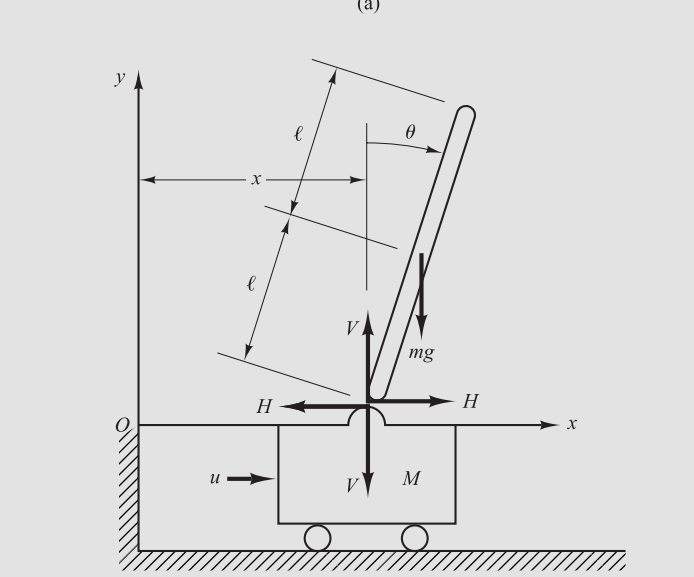
\includegraphics[width=0.7\textwidth]{Imagenes/modelo-pendulo.png}
    \caption{Diagrama del prototipo de péndulo invertido.}
    \label{fig:modelo-pendulo}
\end{figure}

\subsection{Análisis de la barra}

El centro de gravedad de la barra está en el centro geométrico de la misma. Las coordenadas del centro de gravedad de la barra son:

\[
X_{cg} = x + l \sin\theta
\]

\[
Y_{cg} = l \cos\theta
\]

El movimiento rotacional de la barra viene dado por:

\[
\tau = I \ddot{\theta}
\]

donde $I$ es el momento de inercia de la barra alrededor de su centro de gravedad. El movimiento horizontal del centro de gravedad es:

\[
m \frac{d^2}{dt^2}(x + l \sin\theta) = H
\]

El movimiento vertical del centro de gravedad es:

\[
m \frac{d^2}{dt^2}(l \cos\theta) = V - mg
\]

Como se debe mantener el péndulo invertido en posición vertical se puede suponer $\theta$ pequeñas por lo que:

\[
\sin\theta \approx \theta, \quad \cos\theta \approx 1, \quad \dot{\theta}^2 \approx 0
\]

quedan:

\[
(I + ml^2)\ddot{\theta} = mgl\theta - ml\ddot{x}
\]

El momento de inercia en el centro de gravedad es:

\[
\frac{1}{12}mL^2 = \frac{1}{12}m(2l)^2 = \frac{1}{3}ml^2
\]

Sustituyendo en y:

\[
\ddot{\theta} = \frac{3}{4l}g\theta - \frac{3}{4l}\ddot{x}
\]

\subsection{Análisis del carro}

Ya que el actuador es un sistema mecánico el movimiento del carro viene dado por y cuando no se suponen las pérdidas físicas del actuador el sistema está definido por el siguiente juego de ecuaciones:

\[
\ddot{\theta} = \frac{3}{4l}g\theta - \frac{3}{4l}u
\]

\[
\ddot{x} = u
\]

\subsection{Representación en variables de estado}

Con $g = 9.8 \, \text{m/s}^2$:

\[
\dot{\mathbf{x}} = \begin{bmatrix} 0 & 1 & 0 & 0 \\ 0 & 0 & 0 & 0 \\ 0 & 0 & 0 & 1 \\ 0 & 0 & 14.7 & 0 \end{bmatrix} \mathbf{x} + \begin{bmatrix} 0 \\ 1 \\ 0 \\ -1.5 \end{bmatrix} u
\]

\[
\mathbf{y}(t) = \begin{bmatrix} 1 & 0 & 0 & 0 \end{bmatrix} \mathbf{x}(t)
\]

\subsection{Discretizando el sistema con un retenedor de orden cero}

Utilizando un tiempo de muestreo de $T = 0.01 \, \text{seg}$:

\[
\mathbf{x}(n+1) = \begin{bmatrix} 1 & 0.01 & -0.0001 & 0 \\ 0 & 1 & -0.003 & -0.0001 \\ 0 & 0 & 1.0028 & 0.01 \\ 0 & 0 & 0.5659 & 1.0028 \end{bmatrix} \mathbf{x}(n) + \begin{bmatrix} 0.0001 \\ 0.01 \\ -0.0001 \\ -0.003 \end{bmatrix} u(n)
\]

\[
\mathbf{y}(n) = \begin{bmatrix} 1 & 0 & 0 & 0 \end{bmatrix} \mathbf{x}(n)
\]

\subsection{Controlabilidad}

\[
\mathbf{M}_c = \begin{bmatrix} \mathbf{H} & \mathbf{G}\mathbf{H} & \mathbf{G}^2\mathbf{H} & \mathbf{G}^3\mathbf{H} \end{bmatrix}
\]

\[
\mathbf{M}_c = \begin{bmatrix} 0.0001 & 0.0002 & 0.0003 & 0.0004 \\ 0.01 & 0.01 & 0.01 & 0.0099 \\ -0.0001 & -0.0003 & -0.0006 & -0.0011 \\ -0.003 & -0.006 & -0.0091 & -0.0122 \end{bmatrix}
\]

Rango $\mathbf{M}_c = 4$, es controlable.

\subsection{Observabilidad}

\[
\mathbf{M}_o = \begin{bmatrix} \mathbf{C} \\ \mathbf{C}\mathbf{G} \\ \mathbf{C}\mathbf{G}^2 \\ \mathbf{C}\mathbf{G}^3 \end{bmatrix}
= \begin{bmatrix}
1 & 0 & 0 & 0 \\
1 & 0.01 & -0.0001 & 0 \\
1 & 0.02 & -0.0002 & -0.000002 \\
1 & 0.03 & -0.0004 & -0.000006
\end{bmatrix}
\]

Rango $\mathbf{M}_o = 4$, por lo tanto el sistema es observable.
